\documentclass[12pt]{report}

\usepackage[letterpaper, hmargin=0.75in, vmargin=0.75in]{geometry}

\usepackage{
    courier,
    algorithm,
    algpseudocode,
    listings,
    underscore,
    authblk,
    hyperref,
    tikz,
    tabularx,
    float,
    graphicx,
	 color
}

\lstset{basicstyle=\footnotesize\ttfamily}

\setlength{\parindent}{0pt}

\begin{document}

\title{RTX Operating System Software Design Report}

\author{
    Clement Hoang\\
		20531116\\
    \texttt{c8hoang@uwaterloo.ca}
    \and
    David Su\\
		20531116\\
    \texttt{c8hoang@uwaterloo.ca}
    \and
    Cole Vander Veen\\
		20531116\\
    \texttt{@waterloo.ca}
    \and
    Peter Li\\
		20531116\\
    \texttt{@uwaterloo.ca}
}

\date{Winter 2016}

\maketitle


\tableofcontents
\listofalgorithms
\listoffigures

\chapter{Introduction}

% This report is a design document outlining the RTX operating system written by Tyler Babaran, Kelly McBride, and Peter Socha as part of the SE 350 course at the University of Waterloo. The OS is written for an MCB1700 board with an LPC1768 microcontroller.\\
%
% The purpose of this report is to provide documentation on the operating system. It will outline the kernel API available to anyone programming processes for the OS. The provided system and user processes are described in detail. Information on initialization and interrupts it also included. Finally, there is a section describing the time performance of the some of the key kernel primitives.\\
%
% The ruling concept of the RTX detailed here is simplicity. Some of the methods used
% to achieve `simplicity' are unconventional, but the idea of simplicity still holds
% true. The priority queues are implemented as sorted linked lists where high priority
% processes are placed first, the memory heap is implemented in a way that might
% take a few explanations, and the message-envelope structure may seem unconventional,
% but each part is simple enough and they are separate concerns so that when the RTX
% functions, every part functions together as a whole in a simple and expected way.

The purpose

\chapter{Design Description}

\section{Data Structures}
\begin{itemize}
  \item \texttt{MemBlock}: a node that represents a block of memory, with its size defined by the global, \texttt{BLOCK_SIZE}
  \item \texttt{MemQueue}: a data structure which models the physical memory available to the OS, using a linked list of \texttt{MemBlock} nodes.

  \item \texttt{PCB}
  \item \texttt{PCBQ}
  \item \texttt{envelope}
  \item \texttt{gp_pcbs}
\end{itemize}

\section{Global Variables}
\begin{itemize}
  \item \texttt{memQueue}:
  \item \texttt{gp_pcbs}:
  \item \texttt{gp_stack}
  \item \texttt{p_end}
  \item \texttt{numOfBlocks}
\end{itemize}

\section{Memory Management}

\subsection{Memory Structure}

dsfdasfdsafdsafdsafsadfdsaf

\begin{figure}
	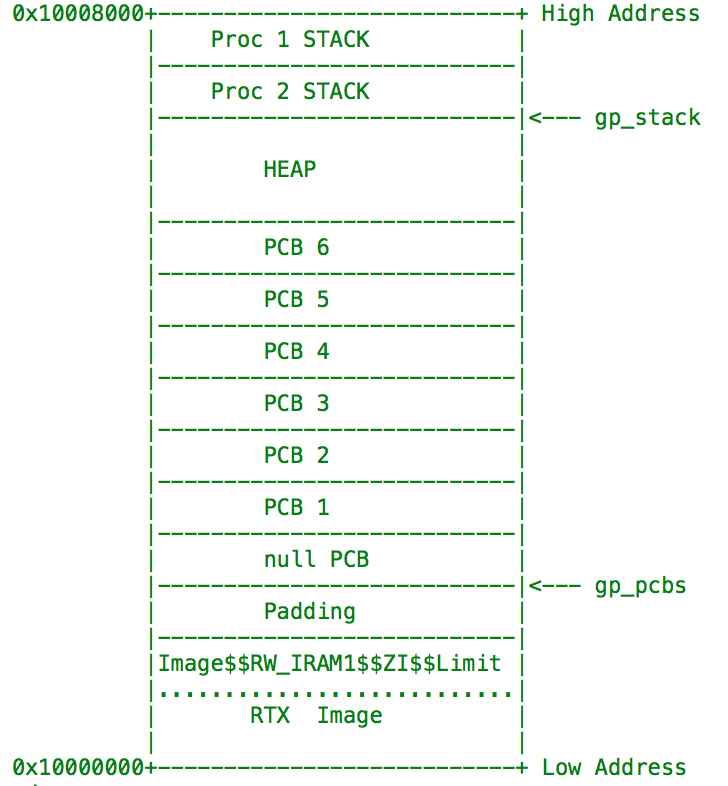
\includegraphics{memory.png}
\caption{Memory Layout}

\end{figure}

\subsection{Requesting Memory Blocks}

\begin{minipage}{\textwidth}
\begin{lstlisting}[language=C, frame=single]
int k_request_memory_block(void);
\end{lstlisting}
\end{minipage}

describe input, output, effects

\begin{algorithm}
  \caption{k_request_memory_block}
  \begin{algorithmic}[1]
    \Procedure{request\_memory\_block}{}
      \While{heap is full}
			\State {block the current process}
	  \EndWhile
	  \State {update the free space list}
	  \State {return the address of the top of the block}
    \EndProcedure
  \end{algorithmic}
\end{algorithm}

\subsection{Releasing Memory Blocks}

\begin{minipage}{\textwidth}
\begin{lstlisting}[language=C, frame=single]
int k_release_memory_block(void* memory_block);
\end{lstlisting}
\end{minipage}

describe input, output, effects

\begin{algorithm}
  \caption{The memory release function}
  \begin{algorithmic}[1]
    \Procedure{release\_memory\_block}{*memory_block}
      \If{this block is the top block of the heap}
			\State {modify heap header node (never gets overwritten)}
	  \EndIf
	  \If{there is free space immediately beneath this block}
			\State {combine them by increasing this block's length}
	  \Else { this block becomes a new block node, is added to the list}
	  \EndIf
	  \If{there is free space immediately beneath this block}
			\State {combine them by increasing this block's length}
	  \EndIf
	  \If{a process is blocked on memory}
			\State {unblock that process, release the processor}
	  \EndIf
    \EndProcedure
  \end{algorithmic}
\end{algorithm}

\pagebreak


%%%%%%%%%%%%%%%%%%%%%%%%%%%%%%%%%%%%%%%%%%%%%%%%%%%%%%%%%%%%%

\section{Processor Management}

\subsection{Process Control Structures}
DFASFAFD

\subsection{Process Queues}

fsadfasdfadsf

\subsection{Process Scheduling}
sdfasdfasdfdasf

%%%%%%%%%%%%%%%%%%%%%%%%%%%%%%%%%%%%%%%%%%%%%%%%%%%%%%%%%%%%%

\section{Process Priority Management}

\subsection{Get Process Priority}

asdfadsfasf

\subsection{Set Process Priority}

dsfasdfasfsfdf

%%%%%%%%%%%%%%%%%%%%%%%%%%%%%%%%%%%%%%%%%%%%%%%%%%%%%%%%%%%%%

\section{Interprocess Communication}

\subsection{Message Structure}

dsfadsfadsfdasfdafs

\subsection{Sending Messages}

adsfdsafasdfasf

\subsection{Receiving Messages}

dsfafasfdasf

\subsection{Delayed Send}


sdfasfasfd

%%%%%%%%%%%%%%%%%%%%%%%%%%%%%%%%%%%%%%%%%%%%%%%%%%%%%%%%%%%%%

\section{Interrupts and I-Processes}

\subsection{UART I-Process}

dsfadsfadsfadsf

\subsection{Timer I-Process}

sdfasfdafd

%%%%%%%%%%%%%%%%%%%%%%%%%%%%%%%%%%%%%%%%%%%%%%%%%%%%%%%%%%%%

\section{System Processes}

\subsection{Null Process}

sdfdasfafadsf

\subsection{CRT Process}

sdfdsfafaf

%%%%%%%%%%%%%%%%%%%%%%%%%%%%%%%%%%%%%%%%%%%%%%%%%%%%%%%%%%%%%

\section{User Processes}

\subsection{Wall Clock Process}

sdfasdfafadf

\subsection{Set Priority Process}

dsfasdfasdfadsf

\subsection{Stress Test Processes}

dfdasfasdfads

\section{Initialization}

dasfasfasfd

\section{Testing}

dfadsfasdf

\chapter{Lessons Learned}

\section{Source Control and Code Management}

sdfdsafsadf

\chapter{Team Dynamics and Individual Responsibilities}

\section{adsfadsf}

dfasfasdf

\chapter{Timing and Analysis}

\end{document}
